\section{Conception du programme} % (fold)
\label{sec:conception}

La parallélisation du programme de lancer de rayons s'est faite en plusieurs étapes. Le programme se compose d'une scène qui est elle-même séparée en carreaux (aussi nommés tuiles ou tâches). Chaque carreau correspond à un carré de pixels. Le calcul de chaque carreau est indépendant du calcul des autres carreaux. Grace à cette propriété, il est possible de paralléliser le programme uniquement en s'occupant de la répartition du calcul des carreaux. La bibliothèque MPI sera utilisée pour ce travail.\\

Dans un premier temps, nous avons utilisé le théorème des reste chinois pour répartir les carreaux sur les différents processus MPI. Cela permet d'avoir une répartition pseudo aléatoire des carreaux. Pour $P$ processus MPI, le programme est constitué d'un processus principal qui rassemblera le travail des $P-1$ processus secondaires, qui effectueront le calcul des carreaux. Dans un second temps, nous avons séparé la charge de travail au sein des processus secondaires. Nous avons pour cela utilisé les threads POSIX. Chaque processus crée un nombre de threads $t$ défini à l'avance. Le travail des processus est alors séparé entre les threads grace à une file de travail. Chaque thread récupère un carreau à calculer jusqu'à ce que la file soit épuisée.\\

Le théorème des restes chinois répartit de façon équitable le travail en fonction du nombre de carreaux à calculer. Cependant, le temps de calcul des carreaux varie selon la complexité des rayons. Pour équilibrer la charge de calcul entre les processus, nous avons créé un anneau de communication entre les processus secondaires. Lorsqu'un processus n'a plus de travail, il envoie un message sur l'anneau. Si un processus possédant encore du travail à réaliser reçoit une demande de travail, il envoie directement le travail au processus ayant initié la demande. S'il n'a pas de travail à transmettre, il envoie la requête de travail au processus suivant dans l'anneau de communication. Lorsqu'un processus reçoit son propre message de demande de travail, cela signifie que tous les carreaux ont été calculés ou que les derniers carreaux sont en cours de calcul. Il envoie alors un message pour signaler la fin du programme et se termine. Un processus qui reçoit le message de terminaison sait qu'il n'y a plus de travail à effectuer et envoie à son tour le message de terminaison puis se termine une fois le calcul de ses carreaux accompli.

\begin{figure}[H]
\centering
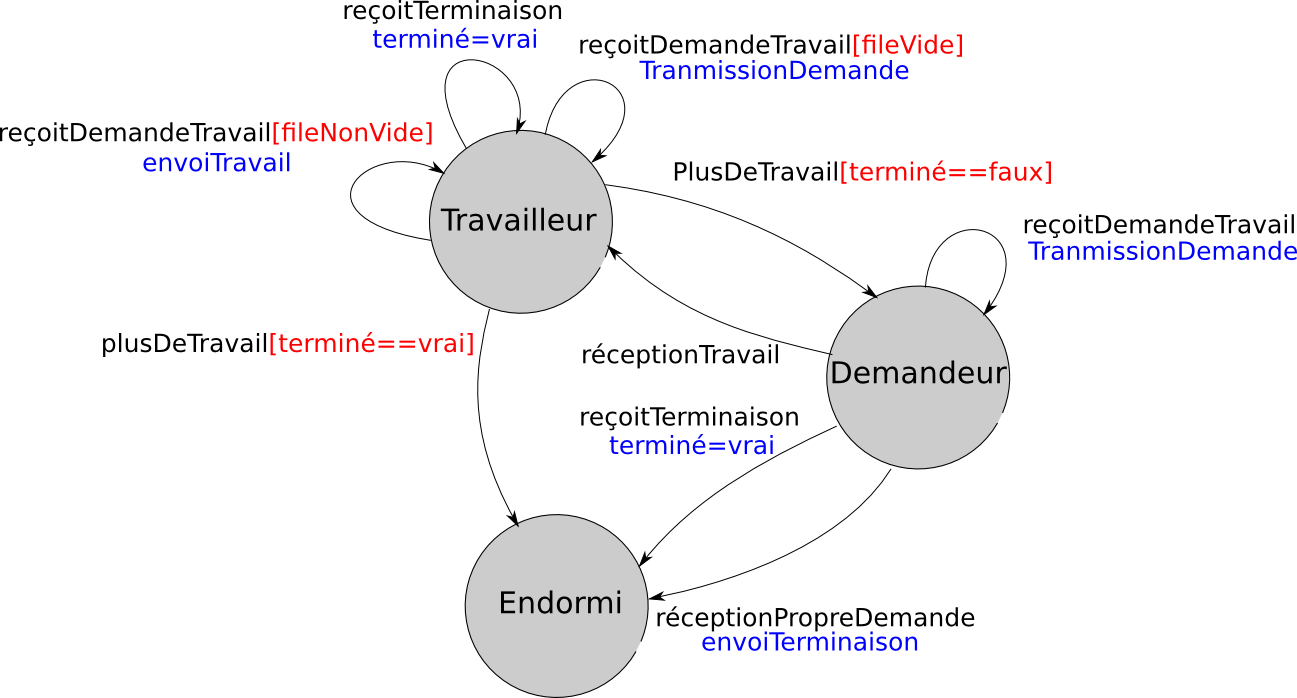
\includegraphics[width=1\textwidth]{automate.png}
\caption{Automate d'un processus secondaire pour les communications réseau}
\label{fig:diff}
\end{figure}

Afin de tester le bon fonctionnement de la transmission des tâches, nous avons implémenté un système de tâches factices permettant de donner aux tâches une longueur variable et déterminée à l'avance contrairement au calcul des carreaux. Le but est de créer un nombre différent de tâches sur chaque processus et de vérifier que la charge de calcul est la même sur chaque processus.

% /section end
